%%=============================================================================
%% Methodologie
%%=============================================================================

\chapter{Methodologie}
\label{ch:methodologie}

%% TODO: Hoe ben je te werk gegaan? Verdeel je onderzoek in grote fasen, en
%% licht in elke fase toe welke stappen je gevolgd hebt. Verantwoord waarom je
%% op deze manier te werk gegaan bent. Je moet kunnen aantonen dat je de best
%% mogelijke manier toegepast hebt om een antwoord te vinden op de
%% onderzoeksvraag.
\section{Redenen}
\label{sec:Redenen}

\section{ Technische voor-en nadelen van Puppet en Ansible}
\label{sec: technische-voor-en-nadelen-van-Puppet-en-Ansible}
Zowel Puppet als Ansible hebben een gelijkaardige infrastructuur, maar verschillen in de deta{\"\i}ls. Om de resultaten van de vergelijkende proef zo betrouwbaar mogelijk te maken is getracht de verschillen tussen beide opstellingen zo minimaal mogelijk te houden. Beide opstellingen zijn dan ook gebasseerd op de infrastructuur die te zien is op afbeelding \ref{fig:infrastructuur}.

In het geval van Puppet zal server A uit afbeelding \ref{fig:infrastructuur} de PuppetMaster zijn. Het is deze server die de puppet manifests bewaart en compileert naar catalogs. Bij Ansible zal deze server AnsibleTower ge{\"\i}nstalleerd hebben en verder bevat deze server uiteraard het ansible equivalent van manifests, playbooks genaamd. 

Server B t.e.m. D stellen de clients voor. Zij ontvangen een bepaalde configuratie van server A om vervolgens de nodige services te installeren en te configureren.

\begin{figure}
  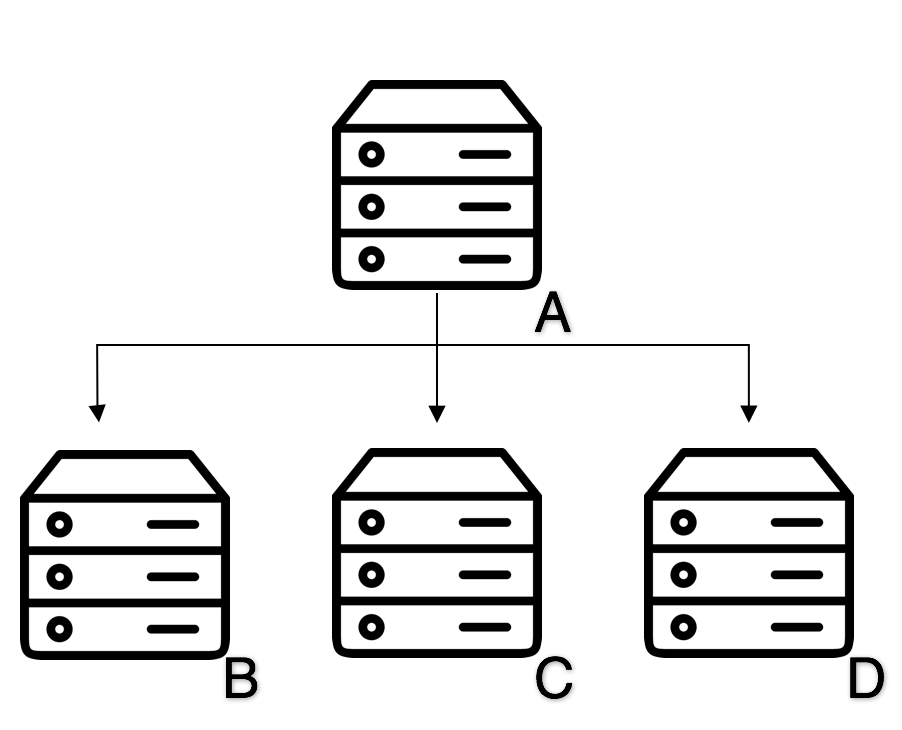
\includegraphics[width=100px]{img/infrastructruur.png}
  \caption{Infrastructuur}
  \label{fig:infrastructuur}
\end{figure}

Om deze opstelling te kunnen verwezelijken en om gelijkheid tussen beide infrastructuren te garanderen werd er gebruik gemaakt van Vagrant. Deze technologie staat ons in staat om eenvoudig servers op te zetten. Vervolgens werden deze servers voorberereid met de nodige configuraties zoals het installeren van de monitoringstool. Het is vanzelfsprekend dat de monitoringstool al opperationeel is alvorens Puppet en Ansible de configuraties overnamen. Want het is juist dit dat gemonitord dient te worden. Daarom is beslist om de configuratie van de monitoringstool door Vagrant uit te laten voeren.


\underline{\textbf{Vagrantfile}} Puppet infrastructuur
\lstinputlisting[language=Ruby]{/Users/thomasdetemmerman/Documents/Bachelorproef-Ansible-vs-Puppet/ProofOfConcept/Puppet/Vagrantfile}

Een woordje uitleg bij deze Vagrantfile:

Lijn 1 en 2 zijn variabelen. 'AmountOfVM' stelt het aantal client VM's voor. In totaal zullen er dus altijd AmountOfVM + 1 virtuele machine aangemaakt worden. Deze '+ 1' is afkomstig van de master welke standaard aangemaakt wordt.

Lijn 4 t.e.m.16 betreffen de master VM, oftwel server A uit afbeelding  \ref{fig:infrastructuur}.
De reden van lijn 14 en 15 is om het probleem op te lossen waarbij de interface, die aangemaakt word op lijn 13, niet automatisch gestart word.

Lijn 18 t.e.m 35 betreffen de clients, oftewel server B, C, D uit afbeelding  \ref{fig:infrastructuur}. Dankzij de variable 'AmountOfVM' kunnen deze dynamisch bijgebouwd worden. 
Lijn 20 t.e.m 22 zorgen ervoor dat alle VM's dezelfde resources ter beschikking krijgen. Deze resources zijn bewust laag gehouden zodat fluctuaties in de monitoringstool beter zouden opvallen.
Lijn 30 en 31 zorgen voor de opstart van het script newrelicinfra.sh. Dit script installeert New Relic, de gekozen monitoringstool. Hiermee zijn we in staat om data  te analyseren vannop het online platform van New Relic.
Lijn 32 en 33 starten het script genaamd installpuppetagent.sh. Hiermee word puppet ge{\"\i}nstalleerd, gestart om vervolgens automatisch een certificaat aan te vragen bij de PuppetMaster. Dit komt omdat alleen gecertificeerde PuppetClients configuraties van de PuppetMaster kunnen ontvangen.

Ondanks er getracht ihet zo gelijk mogelijk te houden zijn er wel enkele kleine verschillen, het blijven immers verschillende technologie\"en.

2 VmGroupName =/ "Anode/" \newline
11 machine.vm.box = /"ansible/tower" \newline
13  machine.vm.network "private\_network", ip: "192.168.100.20" \newline
27  machine.vm.network "private\_network", ip: "192.168.100.\#\{20+machine\_id\}"  \newline
32  \# NIET AANWEZIG\newline
33 \#NIET AANWEZIG\newline

Een eerste belangrijk verschil wordt al in deze vroege fase duidelijk. Namelijk de afwezigheid van installpuppetagent.sh in het geval van de Ansibleinfrastructuur. Opvallend is ook dat hier geen alternatief script voor nodig is. Ansible maakt namelijk geen gebruik van agents. Het installpuppetagent.sh bestaat uit de volgende stappen:

\lstinputlisting[language=Ruby]{/Users/thomasdetemmerman/Documents/Bachelorproef-Ansible-vs-Puppet/ProofOfConcept/Puppet/puppetagent/installpuppetagent.sh}

Hierbij wordt er eerste de repository van Puppet toegevoegd om het vervolgens te installeren. Hierna plaatsen we een niewe hosts file op de server aangezien de afwezigheid van een DNS-server in onze opstelling. Ook wordt de Puppet.conf aangepast. Hierbij voegen we de FQDN van de PuppetMaster toe. Om te eindigen starten we de service en doen we een aanvraag bij de master voor een certificaat.























